\section{Web3} 
web3.js is a collection of libraries that allows you to interact with a local or remote Ethereum node. Moreover, it is able to communicate with MetaMask, which is the add-on for Chrome and Mozilla Firefox that lets the user manage his Ethereum wallet and confirm transactions in an intuitive and secure way. Using MetaMask we offer secure payments and automatic login to \textit{Soldino}.
\subsection{Architecture overview}
To interact with web3 library calls we organized the \texttt{web3functions} package into five different modules:
\begin{figure}[h]
	\centering
	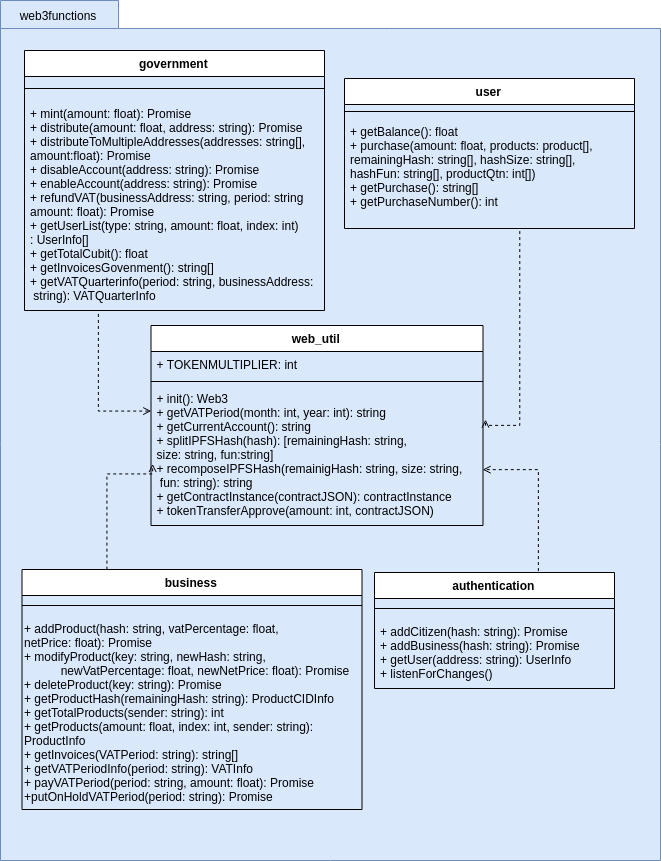
\includegraphics[scale=0.47]{res/images/web3.png}
	\caption{Class diagram of the \texttt{web3functions} package}
\end{figure}
\\Since the programming language used to code this package is JavaScript, the type of many of the methods in the diagram shown above are just JSON with specific fields. In particular:
\begin{itemize}
	\item if the returned type is \texttt{Promise}, the returned type is a Promise that resolves if the function call went well, otherwise rejects with an error message;
	\item the other non-standard types have to be intended as JSON with specific fields and are better explained below, alongside with the description of the first method that uses it.
\end{itemize}
\subsection{Methods and constants}

The five modules groups some methods that are responsible for setting data to Ethereum or retrieving them from the blockchain.

\subsubsection{web\_utils}
This module groups some utility functions that are used by the other modules to make the web3 call easier:
\begin{itemize}
	\item \textbf{init}: tries to get an instance of a web3 object, which will be used to make all the Web3 calls. Specifically, it tries to get the Web3 object (defined by the Web3 library) instance injected by MetaMask\glo, if this is possible, otherwise it returns an error;
	\item \textbf{splitIPFSHash}: a function that converts the base58 string representing the IPFS CID into three variables(object ID, size of the ID, hash function ID), since this information is saved in this way in the blockchain for cost and scalability reasons;
	\item \textbf{recomposeIPFSHash}: it's the inverse of the function described above, it recomposes the IPFS CID starting from the three variables mentioned above;
	\item \textbf{getVATPeriod}: returns the VAT period id starting from the current date. The format is YYYY-Q, where YYYY is the current year, and Q is the current trimester (a value between 1 and 4);
	\item \textbf{getCurrentAccount}: returns the current default account reading it from the current Web3 object instance;
	\item \textbf{getContractInstance}: retrieves an object of the last version instance of the deployed smart-contract related to the parameter passed. The parameter contractJSON is the JSON given as result from the compilation of the desired smart-contract produced with the command \texttt{truffle compile};
	\item \textbf{tokenTransferApprove}: gives the authorization, to the last version instance of the deployed smart-contract related to the parameter passed, to withdraw the specified amount of Cubit\glosp from the current user account;
	\item \textbf{TOKENMULTIPLIER}:     in order to save the decimal numbers in Solidity, since this language does not support only integers, the value passed to and retrieved from Solidity must be multiplied for and divided by this constant. The constant is currently set to 100, in order to save 2 decimal digits.
\end{itemize} 

\subsubsection{authentication\glo}
This module manages the registration and login of all the types of users:
\begin{itemize}
	\item \textbf{listenForChanges}: this function is triggered after the user login. Using the Web3 object injected by MetaMask\glo, it is possible to listen to an event related to account or network changes. In these cases, this function resolves the promise returned that could be used, as we are currently using it, to log out the current user;
	\item \textbf{addCitizen}: registers a new citizen using the Ethereum address provided by MetaMask, and saves the IPFS CID, that represents the related information saved in the peer-to-peer\glosp network;
	\item \textbf{addBusiness}: registers a new business using the Ethereum address provided by MetaMask, and saves the IPFS CID, that represents the related information saved in the peer-to-peer network;
	\item \textbf{getUser}: retrieves the information related to the current account from Solidity. In particular, the UserInfo type returned corresponds to a JSON with the following fields:
	\begin{itemize}
		\item the IPFS hash;
		\item the state of the user (a boolean that indicated if the user is enabled or disabled);
		\item the user type:
		\begin{itemize}
			\item 0: not registered;
			\item 1: citizen
			\item 2: business
			\item 3: government.
		\end{itemize}
	\end{itemize}
\end{itemize}
\subsubsection{user}
This module manages the common functionality offered to citizen and business:
\begin{itemize}
	\item \textbf{getBalance}:returns the Cubit\glosp balance of the current user account;
	\item \textbf{purchase}: manage a new order making the user transfer the due amount of Cubit\glosp to the target companies;
	\item \textbf{getPurchase}: gets the IPFS CID related to the purchases of the current user;
	\item \textbf{getPurchaseNumber}: gets the number of purchases carried out from the current user.
\end{itemize}
\subsubsection{business}
This module manages the functionality offered to business:
\begin{itemize}
	\item \textbf{addProduct}: inserts the product passed as JSON in the Ethereum blockchain; 
	\item \textbf{modifyProduct}: allows a business to modify one of its product that was previously been added;
	\item \textbf{deleteProduct}: allows a business to delete one of its products that were previously been added. The product will not be shown in the store anymore;
	\item \textbf{modifyProduct}: allows a business to modify one of its product that was previously been added;
	\item \textbf{getProductHash}: get the full IPFS CID of a product starting from the object ID;
	\item \textbf{getSalesInvoices}: returns an array containing all the IPFS CID related to the sales invoices;
	\item \textbf{getTotalProducts}: returns the number of products currently available in the store. If the user sets the "sender" parameter to true, the function will return the number of products available in the store, inserted by the current account (a business);
	\item \textbf{getProducts}: returns an array of arrays with information about the products in the store. Specifically, each array contains the IPFS CID of the product, the product's seller and the product ID. If the flag "sender" is set to true, the function returns only the products owned by the logged-in business.
	\item \textbf{getInvoices}: returns an array containing all the IPFS CID related to the business invoices;
	\item \textbf{getVATPeriodInfo}: the function returns the details about the passed VAT period, related to the logged-in business. The returned value (VATInfo) is an array with the following format [businessAddress, state, amount];
	\item \textbf{payVATPeriod}: allows a business to pay the VAT owed to the government related to a particular VAT quarter;
	\item \textbf{putOnHoldVATPariod}: allows a business to postpone of a month the VAT payment to the government related to a particular VAT quarter.
	
\end{itemize}
\subsubsection{government}
Module to manage the common functionality offered to the government:
\begin{itemize}
	\item \textbf{mint}: lets the government mint a specific amount of \textit{Cubit}. This amount is deposited in the government account;
	\item \textbf{distribute}: lets the government transfer a specific amount of \textit{Cubit} from his own account to a target account;
	\item \textbf{distributeToMultipleAddresses}: lets the government transfer a specific amount of Cubit from his own account to each of the accounts in the targets list passed to the function;
	\item \textbf{disableAccount}: lets the government set the state of the target account to "disabled". The target account will not be able to use the platform until it has been restored;
	\item \textbf{enableAccount}: lets the government set the state of the target account to "enabled". The target account will be able to use the platform;
	\item \textbf{refundVAT}: lets the government refund a business. The owed amount of Cubit, related to a specific VAT quarter, will be transferred to the target business;
	\item \textbf{getUserList}: returns an array containing \texttt{amount} JSON with the users' data, skipping the first \texttt{amount*index} users. The user type is the one passed to the function. The JSON (the UserInfo type in the diagrams above) contains all the information inserted by the user in the registration process, plus the state of abled/disabled;
	\item \textbf{getTotalCubit}: returns the total amount of Cubit that was minted in Soldino;
	
	\item \textbf{getInvoicesGovernment}: lets the government refund a business. The owed amount of Cubit, related to a specific VAT quarter, will be transferred to the target business;
	
	\item \textbf{getVATQuarterInfo}: Return the following info about the VAT period:
	\begin{itemize}
		\item businessAddress;
		\item state of the period: [DUE, OVERDUE, PAID, TO\_BE\_REFUNDED, REFUNDED] enum 0->4;
		\item amount: VAT amount of the period.
	\end{itemize} 
\end{itemize}
\subsection{How to extend with new features}
This package should be extended if new interactions with the blockchain are necessary. In fact, this package has the responsibility to interact with the smart-contract. In particular, these modules should be used to save or read the information from the blockchain. Before adding new features we suggest to check the following advice:
\begin{itemize}
	\item the generic functions, such as utility functions, that will concern the different type of user, should be added in the \texttt{web\_util} module;
	\item if the new functionality concerns a particular type of user, it should be added in the suitable existing module. In particular, the \texttt{user} module should be used for operations that pertain both citizen and business;
	\item this package must not interact with other sources apart from the Ethereum blockchain (e.g., IPFS). In order to group information coming from different sources, the \texttt{facade} package should be used (this package will be explained later).
\end{itemize} 


